As mentioned previously, it's computationally expensive to compute the full Fisher Information. A single matrix for the smallest network from the previous section would already be over 50GB in size. Therefore, to be able to compute and visualize the trace of the NTK, the Fisher Information and the curvature $R$, this section covers the training of one of the simplest possible networks.

\subsection{The network}
The network we will use in this section consists of a single neuron with two inputs, no bias and uses a sigmoid function \cite{ActivationFunctionOverview} as its activation function. This means that we can express the output of the network by 
\begin{equation}
	f_\theta(x,y) = \frac{1}{1+ \exp (-5(\theta_1 x + \theta_2 y))},
\end{equation}
with inputs $x$ and $y$. We added the factor $5$ to make the sigmoid function a bit steeper.




\begin{figure}
	\centering
	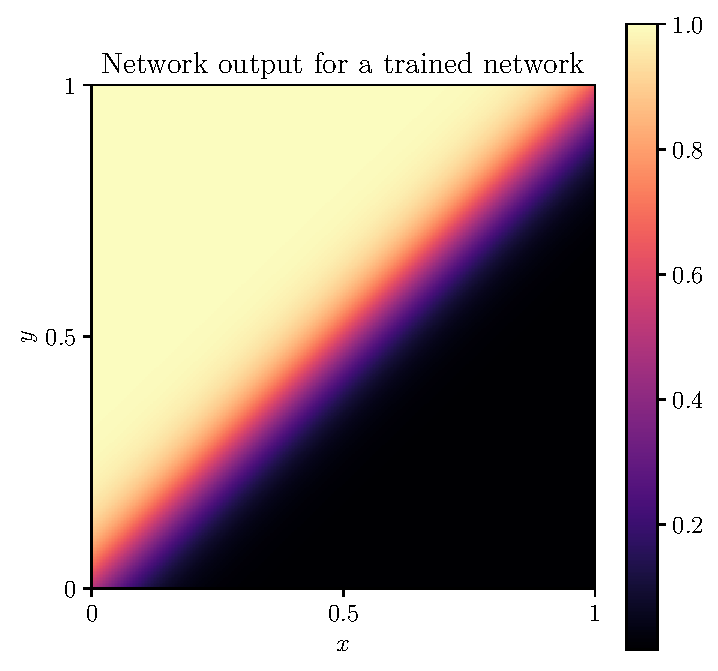
\includegraphics{Experiment2/plots/Network_output.pdf}
	\caption{text}
\end{figure}

\begin{figure}
	\centering
	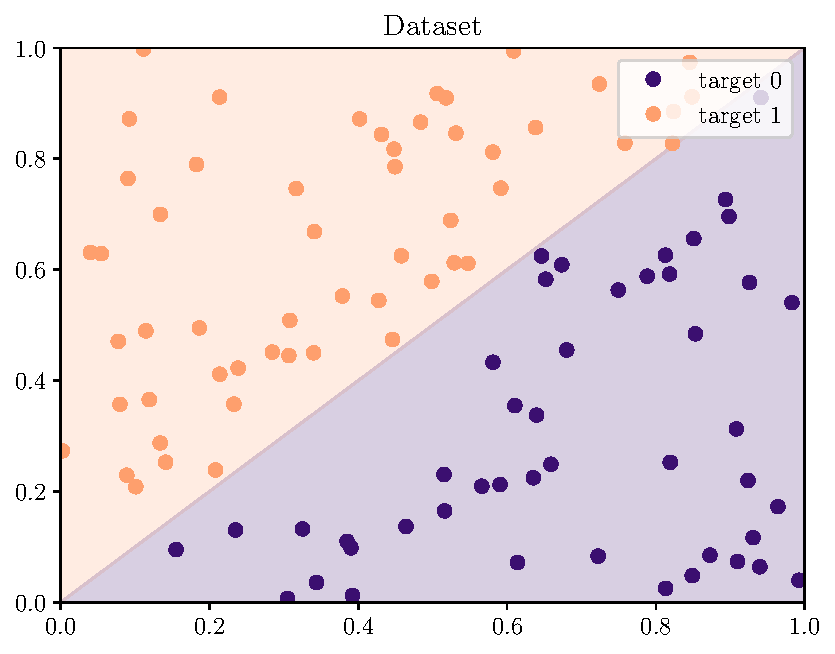
\includegraphics{Experiment2/plots/Dataset.pdf}
	\caption{text}
\end{figure}

\begin{figure}
	\centering
	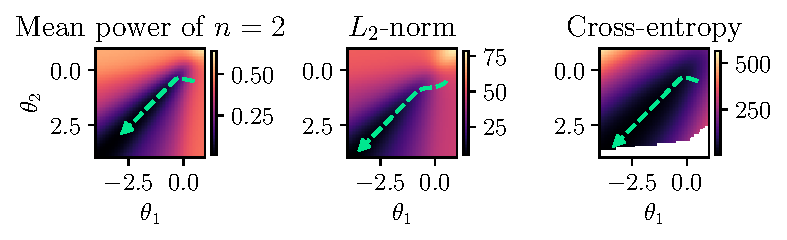
\includegraphics{Experiment2/plots/LossSurfaces.pdf}
	\caption{text}
\end{figure}

\begin{figure}
	\centering
	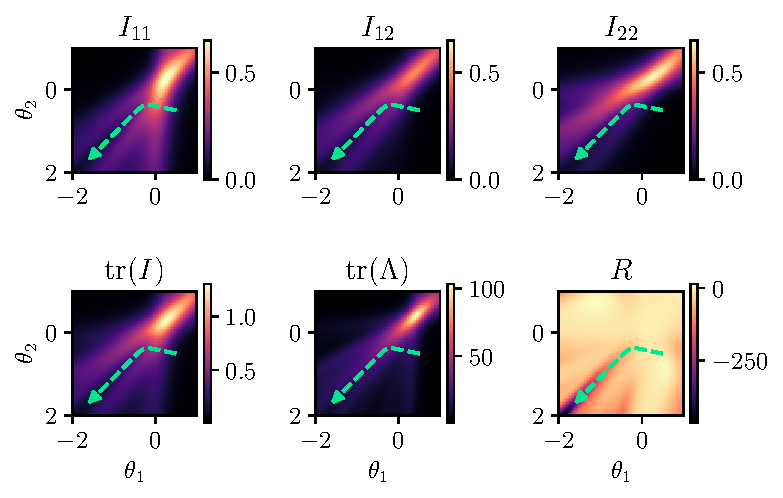
\includegraphics{Experiment2/plots/MeanPowerLoss2_tracecomparison.pdf}
	\caption{text}
\end{figure}

\begin{figure}
	\centering
	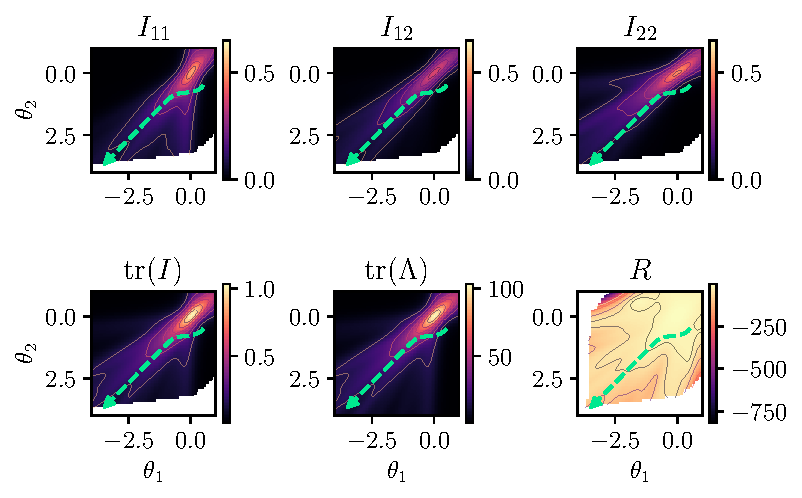
\includegraphics{Experiment2/plots/LPNormLoss2_tracecomparison.pdf}
	\caption{text}
\end{figure}

\begin{figure}
	\centering
	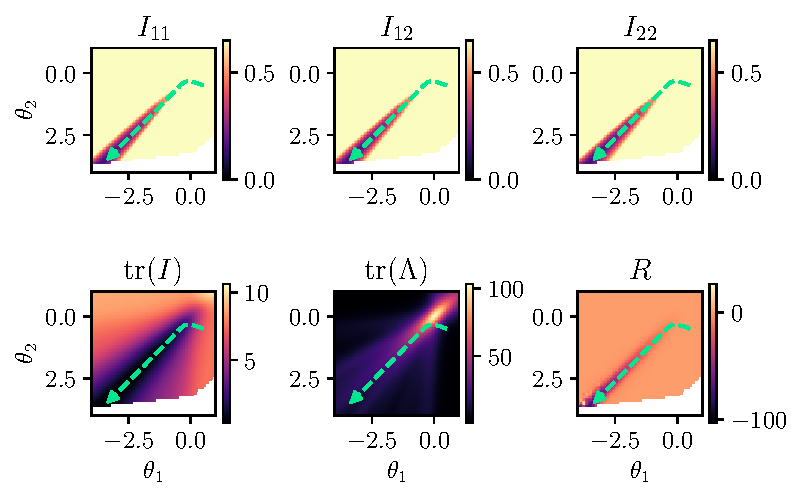
\includegraphics{Experiment2/plots/CrossEntropyLoss_tracecomparison.pdf}
	\caption{text}
\end{figure}

\begin{figure}
	\centering
	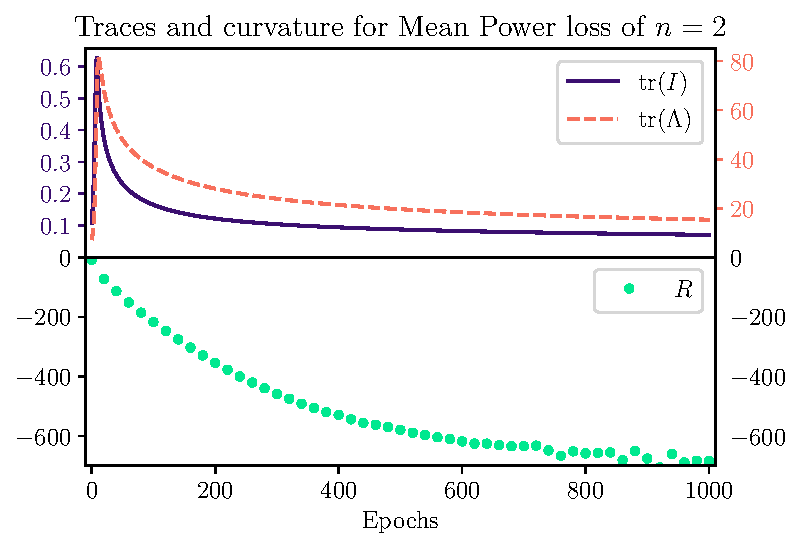
\includegraphics{Experiment2/plots/MeanPowerLoss2_Curves.pdf}
	\caption{text}
\end{figure}

\begin{figure}
	\centering
	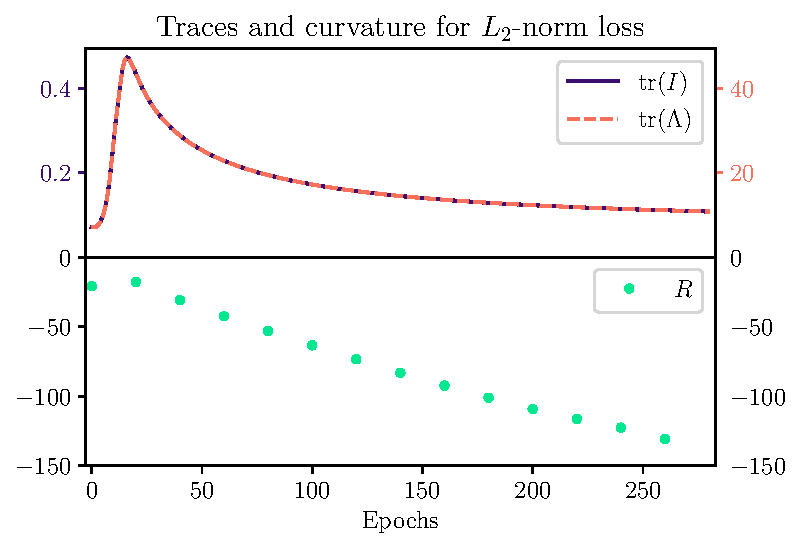
\includegraphics{Experiment2/plots/LPNormLoss2_Curves.pdf}
	\caption{text}
\end{figure}

\begin{figure}
	\centering
	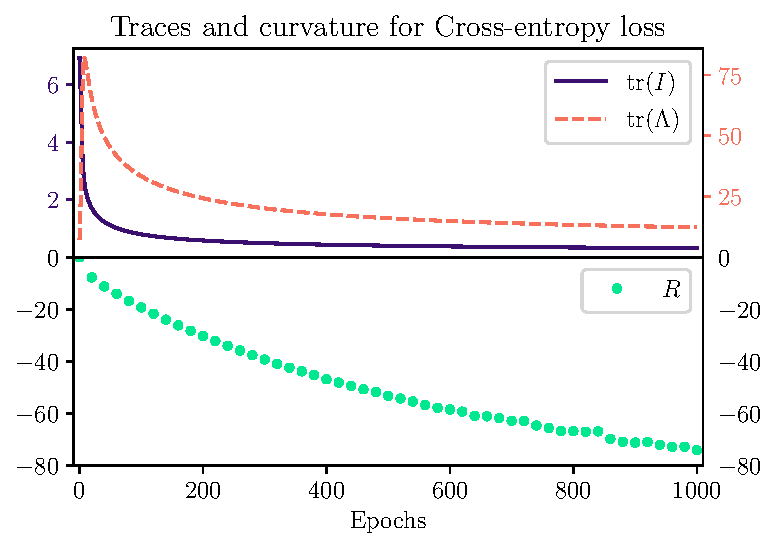
\includegraphics{Experiment2/plots/CrossEntropyLoss_Curves.pdf}
	\caption{text}
\end{figure}